In this section we will deal with the problem of placing side chains
on the protein and selecting side-chain conformations in a way that
minimizes the number of collisions.

As we mentioned in Section \ref{chap:protein_geometry}, statistical
analysis has shown that each type of amino acid side-chain has a small
set of common conformations \cite{dunbrack2002rotamer}. A side-chain
conformation is a configuration of its $\chi$ angles and is called a
\textit{rotamer}.

There has been developed several \textit{rotamer libraries}
\cite{dunbrack1997bayesian, lovell2000penultimate}, containing lists
of the common rotamers for each side-chain together with a probability
of each of those rotamer occuring in a protein. A comparison of some
(but not the most recent) rotamer libraries can be found in
\cite{dunbrack2002rotamer}. We have selected to use the rotamer
library made by Dunbrack et al. for the SCWRL side-chain
predictor\footnote{We use the latest release from 15th May 2002}.

\section{Our approach}
We have devised a simple algorithm for selecting side-chain rotamers
with the goal of minimizing the number of collisions between
atoms. Our first step is to apply the rotamer from the rotamer library
with highest probability to each amino in the protein. After this, we
go through each amino acid, this time trying to eliminate eventual
collisions. We use a breadth-first search through a tree that
represents the eventual collisions occuring for the different rotamers
of the amino acids. On Figure \ref{fig:rotamer-search-tree} we have
illustrated how our algorithm progresses, when trying to remove
collisions with a single amino acid. Each vertex represents an amino
acid and each edge represents a collision between the node and its
child. The names on the edges represents rotamers of the node
above. As an example, when rotamer \textit{k} is applied to amino acid
\textit{a}, \textit{a} collides with both \textit{c} and \textit{d}
(with their current rotamer, remember that we start by selecting the
most likely rotamer for all residues).

%% Hvornår kigger vi på rotameren som a startede ud med at have?

\begin{figure}
	\centering
	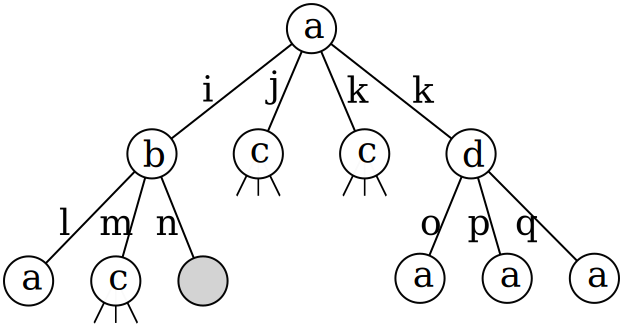
\includegraphics[width=.9\columnwidth]{figures/rotamersearch}
	\caption{The structure of our rotamer search space when eliminating
      collisions with the amino acid \textit{a}.}
    \label{fig:rotamer-search-tree}
\end{figure}

\section{Related Work}
The side-chain placement problem has been investigated by several
research groups, what we found most notably is the work done by
Dunbrack Labs on the SCWRL project \cite{canutescu2003graph,
  krivov2009improved}. To limit the search space, the algorithm of
SCWRL starts by removing rotamers with high self-energy from the set
of possible rotamers, as these are unlikely to be selected. Thus, they
need to use an energy function, which we have limited us from in our
project. Their next step is to resolve whether any collisions can be
transformed into disulfide bridges, which are bonds between two cysteine
amino acids from different places on protein but spatially near each
other.

% SCWRL: 
%  * Bruger energiberegning i valget af rotamerer
%  * Tjekker om par af cysteine amino syrer kan danne disulfid broer


% Todo: snak om SCWRL, der tilføjer side-chains på en fastlåst backbone.


%%% Local Variables: 
%%% mode: latex
%%% TeX-master: "rapport"
%%% End: 
